\chapter{Introduction}
\label{cha:introduction}

% \chapterquote{I'm awesome!}{Barney Stinson, WIRED magazine, 19.1.2009}

\section{Background}

As companies and consumers increasingly purchase goods online, the demand for cross carrier management platform
delivery services grows (First Research 2013, 7). Furthermore, the growth of online retail
sales has influenced the logistics industry for the past ten years and the trend is expected to
continue at least on a similar level during the next few years. (Delfmann et al. 2002, 203.) 

\begin{figure}[!ht]
	\centering
	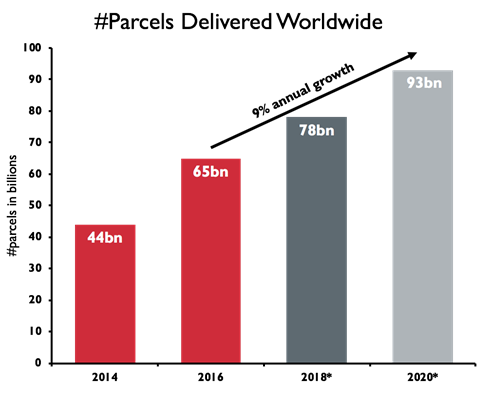
\includegraphics[width=0.5\textwidth]{images/ParcelsDel.png}\\
	\caption{Parcels Delivered worldwide [billions]}
	\label{fig:introduction__loremipsum}
\end{figure}

Responding to the increased demand of small-sized frequent shipments incurred by e-commerce has become one of the biggest challenges for logistics express delivery companies.
A successful delivery of shipments to consumers distributed across large geographical areas
will require re-designing of the existing system.

The increase of business-to-consumer (B2C) e-commerce activities implies that business are border less, global ecommerce is selling products or offer services across the world, in many case without anyu


The idea to investigate delivery service based on the  blockchian proposed by the the Tu Berlin. The DC3 team in this project did not focused in implementing the blockchian system but rather in creating a platform interface to manage the parcel. as today each company store the parcel data in her own local servers, only basic parcel data    






\section{Problem Discussion}

as today each company store the parcel data in her own local servers, only basic parcel data  

\begin{table}[!ht]
	\small
	\centering
	\begin{tabular}{|l|l|l|l|}
		\hline
		Lorem & ipsum & dolor & sit \\
		\hline
		amet & consetetur & sadipscing & elitr \\
		\hline
		Lorem & ipsum & dolor & sit \\
		\hline
		amet & consetetur & sadipscing & elitr \\
		\hline
	\end{tabular}
	\caption{Lorem ipsum...}
\end{table}

alon

\subsection{Lorem ipsum continued}

alon

\subsubsection{Even more Lorem Ipsii}

alon
